%% Requires compilation with XeLaTeX or LuaLaTeX
\documentclass[10pt,xcolor={table,dvipsnames},t]{beamer}
\usetheme{diapo}
\usepackage{amsmath}

\title[Your Short Title]{Lorenz System Project}
\subtitle{Presentation (version 0)}
\author[name]{AYDOGDU Melissa, LECOURTIER Frédérique}
\institute{\large Strasbourg University}
\date{05 april 2022}

\useoutertheme{miniframes}

\begin{document}

\begin{frame}
  \titlepage
\end{frame}

\AtBeginSection[]{
  \begin{frame}
  \vfill
  \centering
  \begin{beamercolorbox}[sep=5pt,shadow=true,rounded=true]{subtitle}
    \usebeamerfont{title}\insertsectionhead\par%
  \end{beamercolorbox}
  \vfill
  \end{frame}
}



\section{Introduction}


\begin{frame}{Examples of application}
    
    Some examples of commonly used commands and features are included, to help you get started.
    \begin{itemize}
      \item Your introduction goes here!
      \item Use \texttt{itemize} to organize your main points.
    \end{itemize}

\end{frame}

\begin{frame}{Lorenz system}
    
    The system :
    $$\left\{\begin{aligned} 
    x'&=\sigma(y-x) \\
    y'&=x(r-z)-y \\
    z'&=xy-bz
    \end{aligned}\right.$$

\end{frame}


\begin{frame}{Goals of the project}
    
    Some examples of commonly used commands and features are included, to help you get started.
    \begin{itemize}
      \item Your introduction goes here!
      \item Use \texttt{itemize} to organize your main points.
    \end{itemize}

\end{frame}


\section{Some interesting properties}

\begin{frame}{Lorenz Attractor}
	
	\begin{figure}[h]
		\begin{minipage}[c]{.46\linewidth}
			\centering
			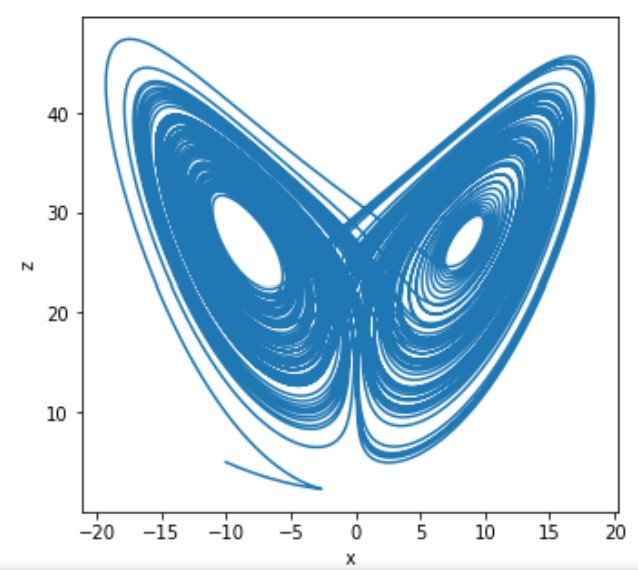
\includegraphics[width=\textwidth]{images/butterfly.jpg}
		\end{minipage}
		\hfill
		\begin{minipage}[c]{.46\linewidth}
			\centering
			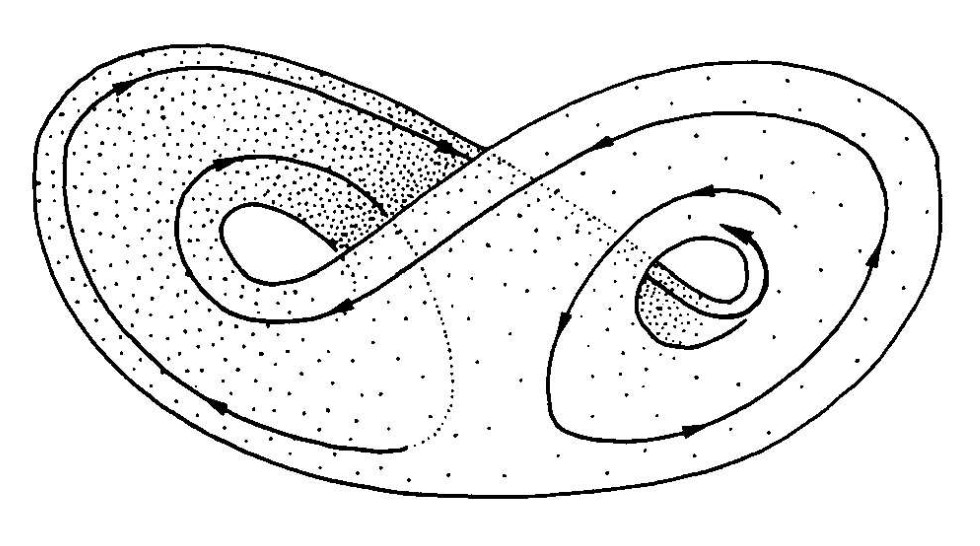
\includegraphics[width=\textwidth]{images/butterfly3D.jpg}
		\end{minipage}
	\end{figure}
	
\end{frame}

\begin{frame}{Chaos theory}

    Some examples of commonly used commands and features are included, to help you get started.
    \begin{itemize}
      \item Your introduction goes here!
      \item Use \texttt{itemize} to organize your main points.
    \end{itemize}

\end{frame}

\section{Numerical resolution with different methods}

\begin{frame}[allowframebreaks]{Methods used to solve Lorenz system}
    
    $f : [0; T] \times \mathbb{R}^n \rightarrow \mathbb{R}^n$, \; a continuous function.

    For $X_0\in \mathbb{R}^n$, we're searching $X\in C^1([0,T],\mathbb{R}^n)$ a solution for :

    $$\left\{\begin{aligned}
        X'&=f(t,X) \\
        X(0)&=X_0
    \end{aligned}\right.$$

    To solve the Lorenz problem we will have:
    
    $$X'=\begin{pmatrix}
        x' \\
        y' \\
        z'
    \end{pmatrix}, \quad X=\begin{pmatrix}
        x \\
        y \\
        z
    \end{pmatrix} \quad et \quad f(t,X)=\begin{pmatrix}
        \sigma(y-x) \\
        x(r-z)-y \\
        xy-bz
    \end{pmatrix}$$
    
    \newpage
    
    \begin{itemize}
        \item Discretization : \\
        \quad 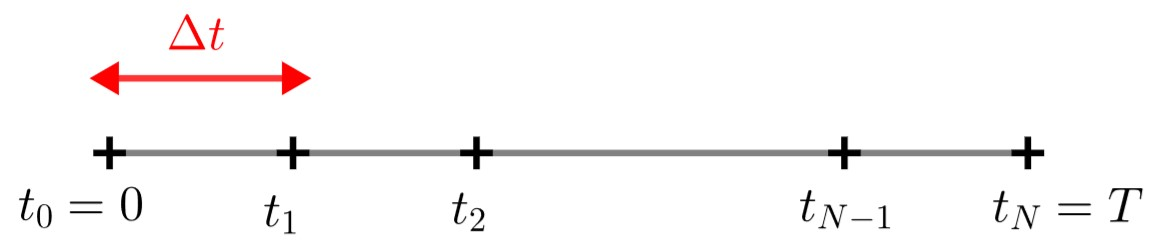
\includegraphics[width=0.4\textwidth]{images/discretization.jpg} \\ 
        Let \quad $t_n=n\Delta t$ \quad with \quad $\Delta t=T/N$ \quad and \quad $X_n=X(t_n)$ \\ \; \\
        \item Euler explicit :
        $$X_{n+1}=X_n+\Delta t f(t_n,X_n)$$
        \item Euler implicit
        $$X_{n+1}=X_n+\Delta t f(t_{n+1},X_{n+1})$$
        
        \newpage
        
        \item Runge Kutta order 4th : \qquad
        $X_{n+1}=X_n+\frac{\Delta t}{6}\left(K_1+2K_2+2K_3+K_4\right)$ \\
        where \qquad $\left\{\begin{aligned}
            K_1&=f(t^n,X^n) \\
            K_2&=f\left(t^n+\frac{\Delta t}{2},X^n+\frac{1}{2} K_1\Delta t\right) \\
            K_3&=f\left(t^n+\frac{\Delta t}{2},X^n+\frac{1}{2} K_2\Delta t\right) \\
            K_4&=f\left(t^n+\Delta t,X^n+K_3\Delta t\right)
        \end{aligned}\right.$ \\ \; \\ \; \\
        
        \item Scipy function : \qquad \textit{scipy.integrate.solve\_ivp}
    \end{itemize}

\end{frame}

\begin{frame}[allowframebreaks]{Some results (with Python)}

    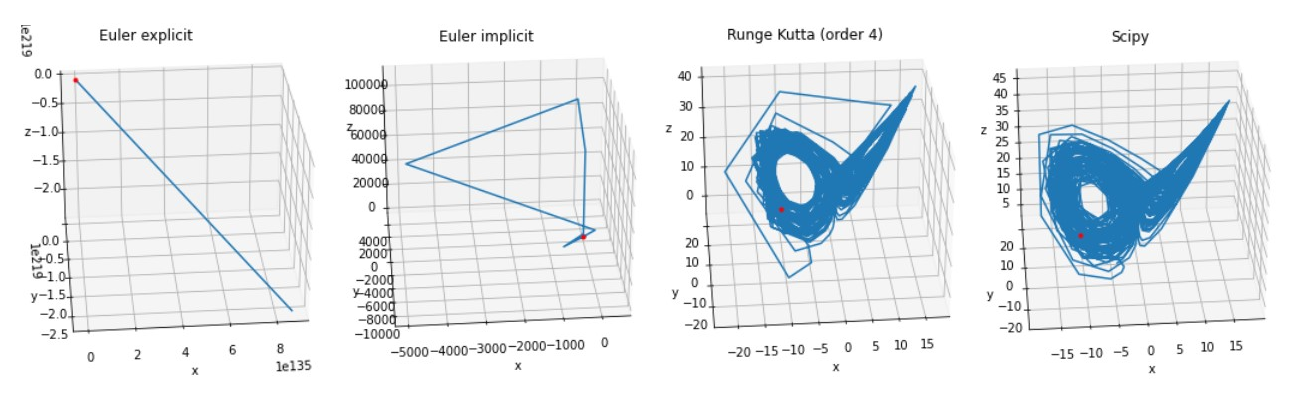
\includegraphics[width=\textwidth]{images/N1000.png} \\ 
    \begin{center}
    	\begin{minipage}[c]{0.5\linewidth}
    		$\sigma=10,\quad \beta=8/3, \quad r=28$ \\
    		$X_0=(-10,10,5)$ 
    	\end{minipage}
    	$T=100, N = 1000 \Rightarrow \Delta t=0.1$
    \end{center}

	\newpage
	
	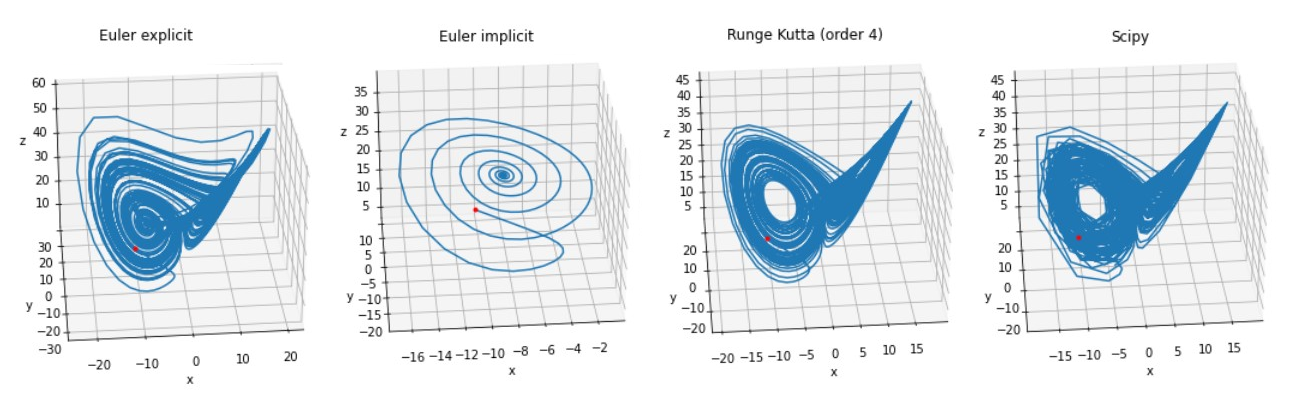
\includegraphics[width=\textwidth]{images/N5000.png} \\ 
	\begin{center}
		\begin{minipage}[c]{0.5\linewidth}
			$\sigma=10,\quad \beta=8/3, \quad r=28$ \\
			$X_0=(-10,10,5)$ 
		\end{minipage}
		$T=100, N = 5000 \Rightarrow \Delta t=0.0.02$
	\end{center}

	\newpage
	
	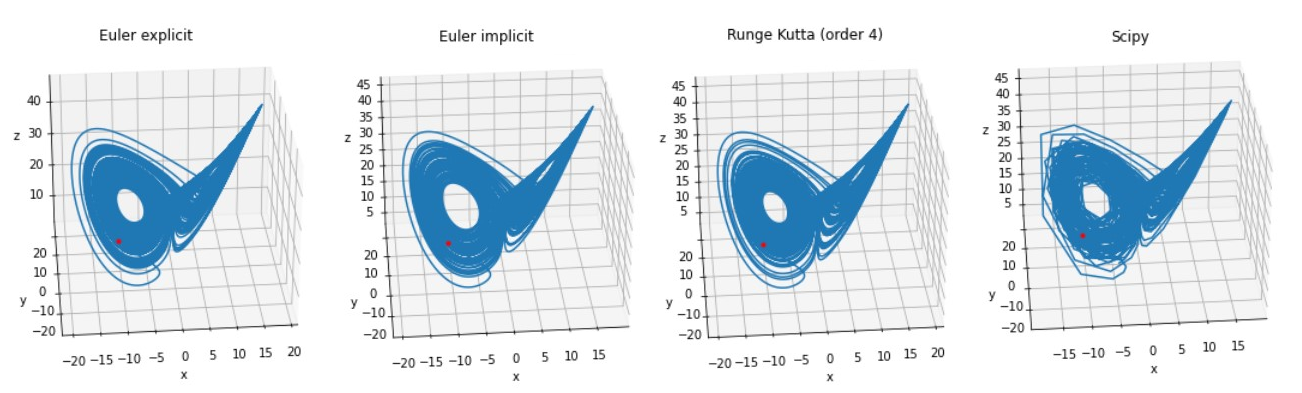
\includegraphics[width=\textwidth]{images/N100000.png} \\ 
	\begin{center}
		\begin{minipage}[c]{0.5\linewidth}
			$\sigma=10,\quad \beta=8/3, \quad r=28$ \\
			$X_0=(-10,10,5)$ 
		\end{minipage}
		$T=100, N = 100000 \Rightarrow \Delta t=0.001$
	\end{center}

	\newpage
	
	\begin{block}{Execution time}
		\; \\
		\begin{center}
			\begin{tabular}{ll}
				Explicit Euler :&  0.003834 \\
				Implicit Euler :&  0.351176 \\
				Runge Kutta :& 0.228595 \\
				Scipy function :&  0.030235
			\end{tabular}
		\end{center}
	\end{block}
    
\end{frame}

\end{document}
